\documentclass[conference]{IEEEtran}
\IEEEoverridecommandlockouts

\usepackage{cite}
\usepackage{amsmath,amssymb,amsfonts}
\usepackage{algorithmic}
\usepackage{graphicx}
\usepackage{textcomp}
\usepackage{xcolor}
\usepackage{booktabs}
\usepackage{url}
\usepackage{hyperref}
\usepackage{microtype}

\hypersetup{
    colorlinks=true,
    linkcolor=black,
    citecolor=black,
    urlcolor=blue
}

\begin{document}

\title{Sim-to-Real Reinforcement Learning for Robust LiDAR-Based Autonomous Navigation: Mid-Term Progress Report}

\author{
\IEEEauthorblockN{Saigirish S}
\IEEEauthorblockA{\textit{Indian Institute of Technology Jodhpur}\\
Roll No: B24ME1066 \\
Email: b24me1066@iitj.ac.in}
\and
\IEEEauthorblockN{Siddhi Vinayak}
\IEEEauthorblockA{\textit{Indian Institute of Technology Jodhpur}\\
Roll No: B24BB1036 \\
Email: b24bb1036@iitj.ac.in}
}

\maketitle

\begin{abstract}
Mapless navigation in dynamic or unstructured environments is a foundational challenge in mobile robotics. While deep reinforcement learning (DRL) provides an end-to-end framework directly mapping onboard sensor observations to continuous velocity commands, standard policies trained in idealized physics engines frequently suffer severe performance degradation when deployed to real hardware due to the reality gap. In this mid-term progress report, we investigate a domain-randomization-enhanced Proximal Policy Optimization (PPO) pipeline for a differential-drive TurtleBot3 mobile robot using a 2D planar LiDAR. We detail the system architecture, comprising a 43-dimensional observation vector with forward-centered sector min-pooling and dead-reckoning pose tracking, safe action scaling, and a multi-component reward formulation. We present preliminary empirical results on a held-out test suite of $N=50$ identical scenarios with static obstacles comparing a nominal baseline policy ($\text{P1}$, 852,816 training steps) against a combined sensor-and-dynamics randomized policy ($\text{P4}$, 704,512 training steps) under nominal evaluation conditions. On nominal testing, $\text{P1}$ achieves a 94.0\% success rate (95\% Wilson score CI: $[83.78\%, 97.94\%]$) while $\text{P4}$ achieves 98.0\% (95\% Wilson score CI: $[89.50\%, 99.65\%]$). A paired McNemar exact test yields $p = 0.6250$, demonstrating that the observed 4.0\% descriptive difference is not statistically significant at $N=50$. We discuss experimental limitations, unequal training budgets, and the necessity of a full $4 \times 4$ policy/environment cross-evaluation matrix to rigorously evaluate perturbation robustness, concluding with a plan toward real-robot transfer conditional on laboratory access.
\end{abstract}

\begin{IEEEkeywords}
Reinforcement Learning, Mobile Robot Navigation, Sim-to-Real Transfer, Domain Randomization, Proximal Policy Optimization, TurtleBot3, ROS 2, Gazebo.
\end{IEEEkeywords}

\section{Introduction and Objectives}
Autonomous ground vehicles operating in GPS-denied indoor environments typically rely on the classical navigation stack consisting of simultaneous localization and mapping (SLAM), global path planning (e.g., A* or Dijkstra), and local trajectory optimization (e.g., Dynamic Window Approach or Timed Elastic Bands) \cite{macenski2020marathon2, macenski2022robot}. While effective in static structured spaces, classical pipelines require substantial computational overhead for real-time dense map maintenance and are notoriously sensitive to localization drift, dynamic obstacle occlusion, and sensor noise \cite{macenski2020marathon2}.

To overcome these constraints, mapless navigation via Deep Reinforcement Learning (DRL) has emerged as an attractive alternative \cite{tai2017virtual}. By training neural network policies to directly map raw range findings and relative goal coordinates to low-level motor velocity commands, the system avoids explicit global mapping. However, training policies directly on physical robotic platforms is prohibitively expensive, wear-intensive, and dangerous during early exploration. High-fidelity simulators such as Gazebo \cite{koenig2004design} provide safe, accelerated experience collection, but policies trained in nominal simulation often experience dramatic performance degradation when transferred to physical hardware---a phenomenon known as the \textit{sim-to-real gap} or reality gap \cite{tobin2017domain, peng2018sim}.

Domain Randomization (DR) bridges this gap by exposing the agent during training to a broad distribution of simulated sensor distortions and unmodeled dynamic variations, compelling the policy to learn robust feedback strategies that generalize across physical discrepancies \cite{tobin2017domain, peng2018sim}. This project systematically investigates the quantitative impact of isolated and combined domain randomization on policy robustness, sample efficiency, and hardware transferability for TurtleBot3 LiDAR navigation.

\subsection{Problem Statement}
We consider a differential-drive ground robot navigating from an arbitrary starting pose $\mathbf{p}_0 = (x_0, y_0, \theta_0)$ to a static Euclidean target $\mathbf{g} = (x_g, y_g)$ in an obstacle-cluttered $4\,\text{m} \times 4\,\text{m}$ bounded workspace. The robot lacks access to a prior global floorplan, external motion capture, or GPS. Navigation must proceed maplessly, relying solely on an onboard 2D laser scanner (LDS-01) and wheel odometry.

\subsection{Research Objectives}
\begin{enumerate}
    \item \textbf{Mapless PPO Navigation Architecture:} Design an end-to-end continuous actor-critic navigation framework operating at 5.0\,Hz that enforces obstacle clearance and smooth kinematic control.
    \item \textbf{$2 \times 2$ Domain Randomization Factorial Design:} Implement modular sensor perturbations (range noise, dropouts, latency, odometry bias) and dynamics perturbations (command gains, actuator lag, control delay, acceleration limits) to isolate their individual and combined effects across four policy regimes:
    \begin{itemize}
        \item $\text{P1}$: Nominal baseline (no randomization).
        \item $\text{P2}$: Sensor randomization only.
        \item $\text{P3}$: Dynamics randomization only.
        \item $\text{P4}$: Combined sensor and dynamics randomization.
    \end{itemize}
    \item \textbf{Rigorous Empirical Benchmarking:} Evaluate trained policies across identical held-out scenarios using paired statistical hypothesis testing and confidence intervals.
    \item \textbf{Physical Sim-to-Real Transfer:} Validate the trained policy without fine-tuning on physical TurtleBot3 hardware in a laboratory environment, conditional on hardware access and safety approval.
\end{enumerate}

\begin{figure*}[t]
\centering
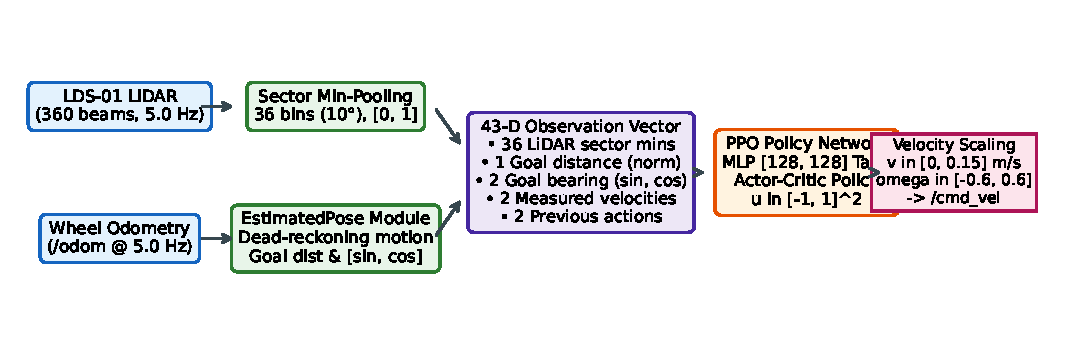
\includegraphics[width=0.92\textwidth]{figures/fig1_system_architecture.pdf}
\caption{System architecture of the mapless PPO navigation framework. Raw 360-beam LiDAR scans are sector min-pooled into 36 forward-centered range bins $[0, 1]$, combined with dead-reckoning goal features from the internal \texttt{EstimatedPose} tracker, velocity feedback, and previous actions into a 43-D observation vector feeding a multi-layer perceptron policy network.}
\label{fig:arch}
\end{figure*}

\section{Planned Methodology and System Design}

\subsection{Observation Space Formulation}
A central failure mode in reinforcement learning is observation distribution shift. To ensure complete parity between simulation and physical deployment, observation preprocessing is implemented as a pure NumPy module (\texttt{ObservationPreprocessor}) with zero ROS dependencies. 

The observation vector $\mathbf{s}_t \in \mathbb{R}^{43}$ is constructed as follows:
\begin{enumerate}
    \item \textbf{LiDAR Sector Min-Pooling ($\mathbf{d}_{0:35} \in [0, 1]^{36}$):} Raw 360-ray range arrays from the LDS-01 sensor ($r_{\min} = 0.12\,\text{m}, r_{\max} = 3.50\,\text{m}$) are pooled into 36 angular sectors of width $10^\circ$. Bin 0 is centered directly forward along the robot's heading ($[-5^\circ, +5^\circ)$). Within each sector, the minimum range is extracted to guarantee conservative obstacle detection, invalid beams ($\le 0$, $\text{NaN}$, $\infty$) are mapped to $r_{\max}$, and values are normalized by $r_{\max}$.
    \item \textbf{Normalized Goal Distance ($d_g \in [0, 1]$):} Relative Euclidean distance to target, normalized by the arena diagonal $D_{\text{arena}} = \sqrt{4^2 + 4^2} \approx 5.657\,\text{m}$.
    \item \textbf{Goal Bearing Representation ($[\sin\phi_g, \cos\phi_g] \in [-1, 1]^2$):} The angular heading error $\phi_g = \text{wrap}(\theta_g - \theta_t) \in [-\pi, \pi]$ is decomposed into its sine and cosine components to eliminate the angular wrap-around discontinuity at $\pm \pi$.
    \item \textbf{Measured Velocity Feedback ($[v_{\text{norm}}, \omega_{\text{norm}}] \in [-1, 1]^2$):} Current measured linear velocity normalized by $v_{\max} = 0.15\,\text{m/s}$ and angular velocity normalized by $\omega_{\max} = 0.60\,\text{rad/s}$.
    \item \textbf{Previous Action Buffer ($\mathbf{u}_{t-1} \in [-1, 1]^2$):} The normalized control vector executed at step $t-1$, providing implicit recurrence and facilitating smooth rate transitions.
\end{enumerate}

\subsection{Dead-Reckoning Estimated Pose Module}
Unlike naive simulations that feed ground-truth simulator poses into the policy, our framework implements an internal \texttt{EstimatedPose} dead-reckoning tracker. At episode reset, the estimated frame is aligned with the initial robot pose. During navigation, measured velocities $(v_{\text{meas}}, \omega_{\text{meas}})$ are integrated over $dt = 0.20\,\text{s}$ using midpoint circular arc kinematics:
\begin{equation}
\theta_{t+1} = \text{wrap}(\theta_t + \omega_{\text{meas}} dt)
\end{equation}
\begin{equation}
x_{t+1} = x_t + v_{\text{meas}} dt \cos\left(\theta_t + \frac{1}{2}\omega_{\text{meas}} dt\right)
\end{equation}
\begin{equation}
y_{t+1} = y_t + v_{\text{meas}} dt \sin\left(\theta_t + \frac{1}{2}\omega_{\text{meas}} dt\right)
\end{equation}
Goal features are computed strictly relative to this estimated frame, faithfully capturing accumulating odometry drift.

\subsection{Action Space and Velocity Scaling}
The policy outputs a continuous action $\mathbf{u}_t = [u_0, u_1]^T \in [-1, 1]^2$. To prevent violent dynamic wear on the physical robot, the active environment implements an asymmetric linear and symmetric angular velocity mapping:
\begin{equation}
v_t = 0.075 \cdot (u_0 + 1.0) \in [0.0, 0.15]\,\text{m/s}
\end{equation}
\begin{equation}
\omega_t = 0.60 \cdot u_1 \in [-0.60, 0.60]\,\text{rad/s}
\end{equation}
This formulation constrains the robot to purely forward motion ($v \ge 0$), preventing backward blind-spot collisions since the LDS-01 sensor possesses structural blind shadows on the rear chassis.

\subsection{Reward Design and Episode Termination}
The step reward function $R_t$ is formulated to provide dense shaping while maintaining high terminal incentives:
\begin{equation}
R_t = r_{\text{progress}} + r_{\text{step}} + r_{\text{goal}} + r_{\text{collision}}
\end{equation}
\begin{itemize}
    \item \textbf{Progress Reward:} $r_{\text{progress}} = 10.0 \cdot (d_{t-1} - d_t)$, providing continuous potential-based gradient toward the goal.
    \item \textbf{Per-Step Penalty:} $r_{\text{step}} = -0.05$, incentivizing time-optimal trajectory completion.
    \item \textbf{Goal Bonus:} $r_{\text{goal}} = +100.0$ when the Euclidean distance to target satisfies $d_t \le 0.20\,\text{m}$ (absorbing terminal state).
    \item \textbf{Collision Penalty:} $r_{\text{collision}} = -100.0$ upon collision.
\end{itemize}
In accordance with standard Gymnasium semantics \cite{towers2023gymnasium}, reaching the goal or colliding triggers \texttt{terminated=True}. If the episode reaches the maximum horizon of $T_{\max} = 350$ steps (70.0\,s) without goal arrival or collision, \texttt{truncated=True} is triggered, ensuring correct value function bootstrapping without treating truncation as an absorbing failure state.

\subsection{Collision Detection Definition Discrepancy}
An important technical distinction arises regarding collision detection:
\begin{itemize}
    \item \textbf{Training Environment (\texttt{tb3\_navigation\_env.py}):} Implements ground-truth geometric contact (\texttt{\_check\_collision()}), verifying whether the robot's circular footprint ($r_{\text{robot}} = 0.105\,\text{m}$) intersects the arena perimeter wall limits ($|x|, |y| \ge 1.95 - 0.105\,\text{m}$) or active obstacle bounding boxes.
    \item \textbf{Standalone Inference Node (\texttt{ppo\_inference\_node.py}):} Lacks access to simulator ground truth or external motion capture. Consequently, it employs a \textbf{LiDAR-range collision proxy}, triggering a safety stop if $\min(\text{ranges}) < 0.16\,\text{m}$.
\end{itemize}
This discrepancy is noted as an operational limitation: while ground-truth geometry governs simulation training, autonomous deployment relies on a conservative sensor-range proxy that may trigger in narrow passages without actual physical contact.

\begin{table}[t]
\caption{PPO Training and Network Hyperparameters}
\centering
\begin{tabular}{llr}
\toprule
\textbf{Category} & \textbf{Hyperparameter} & \textbf{Value} \\
\midrule
Network Arch. & Policy MLP ($\pi$) & $[128, 128]$ \\
              & Value MLP ($vf$) & $[128, 128]$ \\
              & Activation Function & Tanh \\
              & Initial $\log \sigma$ & $-0.5$ \\
\midrule
Optimization  & Algorithm & PPO \cite{schulman2017proximal} \\
              & Learning Rate ($\alpha$) & $3 \times 10^{-4}$ (constant) \\
              & Rollout Length ($n_{\text{steps}}$) & 2048 per worker \\
              & Parallel Workers & 4 \\
              & Minibatch Size & 256 \\
              & Optimization Epochs ($n_{\text{epochs}}$) & 10 \\
              & Discount Factor ($\gamma$) & 0.99 \\
              & GAE Parameter ($\lambda$) & 0.95 \\
              & PPO Clip Fraction ($\epsilon$) & 0.20 \\
              & Entropy Coef. ($c_{\text{ent}}$) & 0.0 \\
              & Value Function Coef. ($c_{\text{vf}}$) & 0.50 \\
              & Gradient Clipping & 0.50 \\
\midrule
Scaling       & Observation Normalization & Fixed Manual ($[0, 1]$) \\
              & Reward Normalization & \texttt{VecNormalize} (returns) \\
\bottomrule
\end{tabular}
\label{tab:hyperparams}
\end{table}

\subsection{Domain Randomization Methodology}
To enforce sim-to-real transferability, we implemented randomized perturbation modules sampled independently at the beginning of each training episode, following principles established in robotics literature \cite{tobin2017domain, peng2018sim}.
\begin{itemize}
    \item \textbf{Sensor Randomization ($\text{P2}$/$\text{P4}$):} Range noise $\sigma(r) = a + b \cdot r$ ($a \in [0.003, 0.015]\,\text{m}, b \in [0.0, 0.010]$), random beam dropout ($p \le 0.05$), contiguous block dropouts (1--2 blocks), delivery latency ($0$ or $0.20\,\text{s}$), and odometry scale/bias drift.
    \item \textbf{Dynamics Randomization ($\text{P3}$/$\text{P4}$):} Command gains $k_v, k_\omega \in [0.85, 1.15]$, actuator lag $\tau \in [0.0, 0.30]\,\text{s}$, control delay $d \in [0.0, 0.20]\,\text{s}$, and acceleration limits ($a_v \in [0.2, 0.6]\,\text{m/s}^2, a_\omega \in [1.0, 3.0]\,\text{rad/s}^2$).
    \item \textbf{Joint Rejection Constraint ($\text{P4}$):} Enforces $\Delta t_{\text{sensor}} + \Delta t_{\text{control}} \le 0.40\,\text{s}$ to guarantee physical traversability.
\end{itemize}

\section{Implementation and Completed Work}
The software stack runs on ROS 2 Humble \cite{macenski2022robot} and Gazebo Classic 11.10.2 \cite{koenig2004design} under Ubuntu 22.04 LTS with PyTorch 2.11.0 (verified from training environment `pip freeze` metadata), Stable-Baselines3 2.7.1 \cite{raffin2021stable}, and Gymnasium 1.2.3 \cite{towers2023gymnasium}.

\subsection{Open-Source Code Repository}
All project source code, simulation environments, training pipelines, observation preprocessors, test suites, and evaluation artifacts are openly hosted on GitHub:
\begin{center}
\url{https://github.com/Saigirish23/tb3-rl-nav}
\end{center}
The repository contains verified implementations of the \texttt{TurtleBot3NavigationEnv}, modular domain randomizers, multi-worker PPO scripts, and the standalone ROS 2 deployment node.

\subsection{Completed Milestones}
\begin{itemize}
    \item \textbf{Simulation Testbed:} Configured Gazebo Classic multi-instance simulation running 4 concurrent headless workers with automated ROS Domain ID isolation and watchdog process recovery.
    \item \textbf{Policy Training Executions:}
    \begin{itemize}
        \item Policy $\text{P1}$ (Nominal baseline): Completed 852,816 transitions over 40,496.33 seconds (11.25 hours). The overall wall-clock throughput is $21.06\,\text{steps/s}$ ($19.75\,\text{steps/s}$ running average reported in run metadata).
        \item Policy $\text{P4}$ (Combined DR): Completed 704,512 transitions over 35,551.54 seconds (9.88 hours). The overall wall-clock throughput is $19.82\,\text{steps/s}$ ($19.69\,\text{steps/s}$ running average reported in run metadata).
    \end{itemize}
    \item \textbf{Standalone Inference Node:} Developed \texttt{ppo\_inference\_node.py}, an asynchronous ROS 2 node executing deterministic policy inference at 5.0\,Hz with integrated sensor watchdog fail-safe.
    \item \textbf{Automated Test Suites:} Verified core functionality using targeted test suites (11/11 passing tests across inference correctness and observation preprocessing) within a broader 69-test automated testing framework.
    \item \textbf{Reward Audit Harness:} Executed a multi-baseline reward audit producing 321,557 lines of per-step reward traces across reactive, random, stationary, and spin-in-place policies.
    \item \textbf{Simulated Multi-Target Demonstration:} Successfully conducted 3 consecutive multi-target navigation trials in Gazebo Classic simulation without collisions or timeouts (3/3 successful trials).
\end{itemize}

\begin{table}[t]
\caption{Preliminary Held-Out Evaluation Results Under Nominal Conditions ($N=50$ Scenarios)}
\centering
\begin{tabular}{lrr}
\toprule
\textbf{Metric} & \textbf{Policy P1 (Nominal)} & \textbf{Policy P4 (Combined DR)} \\
\midrule
Training Steps Completed & 852,816 & 704,512 \\
Training Random Seed & $s=0$ & $s=0$ \\
Evaluation Scenarios ($N$) & 50 & 50 \\
\textbf{Success Count} & \textbf{47 / 50} & \textbf{49 / 50} \\
\textbf{Success Rate} & \textbf{94.0\%} & \textbf{98.0\%} \\
95\% Wilson Score CI & $[83.78\%, 97.94\%]$ & $[89.50\%, 99.65\%]$ \\
Collision Count & 1 / 50 (2.0\%) & 1 / 50 (2.0\%) \\
Timeout Count & 2 / 50 (4.0\%) & 0 / 50 (0.0\%) \\
Mean Steps to Goal (Succ.) & $106.17 \pm 48.2$ & $101.49 \pm 44.8$ \\
Mean Duration to Goal (Succ.) & $21.23 \pm 9.6\,\text{s}$ & $20.30 \pm 9.0\,\text{s}$ \\
Mean Path Length (Succ.) & $2.25 \pm 0.72\,\text{m}$ & $2.07 \pm 0.58\,\text{m}$ \\
Mean Min. Clearance (Succ.) & $0.289\,\text{m}$ & $0.298\,\text{m}$ \\
\midrule
\textbf{Paired McNemar Test} & \multicolumn{2}{c}{\textbf{Exact Two-Sided $p = 0.6250$ (Not Significant)}} \\
\bottomrule
\end{tabular}
\label{tab:results}
\end{table}

\begin{figure*}[t]
\centering
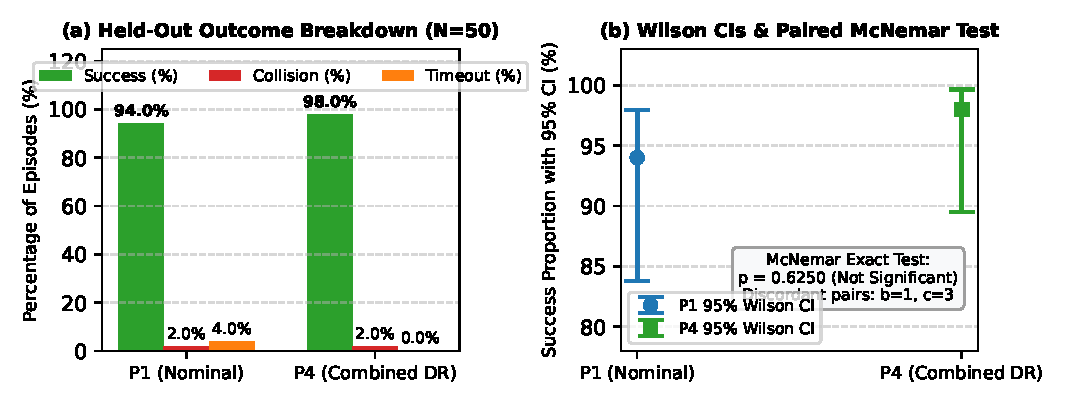
\includegraphics[width=0.92\textwidth]{figures/fig2_evaluation_results.pdf}
\caption{Held-out evaluation outcomes on $N=50$ identical scenarios under nominal evaluation conditions. (a) Outcome distributions showing higher success rate and zero timeouts for $\text{P4}$. (b) Wilson 95\% confidence intervals highlighting substantial interval overlap and the exact two-sided McNemar test result ($p = 0.6250$), demonstrating descriptive improvement without statistical significance.}
\label{fig:results}
\end{figure*}

\section{Preliminary Results and Discussion}

\subsection{Held-Out Scenario Evaluation (Nominal Conditions)}
To evaluate baseline generalization, policies $\text{P1}$ and $\text{P4}$ were benchmarked against a frozen test suite of $N=50$ held-out scenarios with static obstacles (\texttt{scenarios/test/scenarios.json}, SHA-256: \texttt{d9a6a25c...}) under \textbf{nominal evaluation conditions}. Table~\ref{tab:results} summarizes the comparative performance metrics.

Policy $\text{P4}$ achieved 49 successes out of 50 episodes (98.0\%), compared to 47 successes for $\text{P1}$ (94.0\%). Crucially, under nominal conditions, $\text{P4}$ eliminated all episode timeouts (0 vs. 2 for $\text{P1}$), while maintaining identical collision counts (1 collision each). As illustrated in Fig.~\ref{fig:boxplots}, $\text{P4}$ also exhibited marginally superior path efficiency, reaching the goal in an average of $20.30\,\text{s}$ ($101.49$ steps) and $2.07\,\text{m}$ path length, compared to $21.23\,\text{s}$ ($106.17$ steps) and $2.25\,\text{m}$ for $\text{P1}$.

\textbf{Scope of Evaluation:} It is vital to emphasize that this benchmark evaluates performance solely under unperturbed, nominal physics. Consequently, these preliminary results demonstrate nominal navigation competence, but do \textit{not} establish empirical robustness to sensor or dynamics perturbations, nor do they prove sim-to-real transfer.

\subsection{Statistical Interpretation and Rigor}
A critical requirement of scientific reporting is distinguishing descriptive gains from statistical significance. Because both policies were evaluated on identical paired scenario configurations, we evaluated the contingency matrix:
\begin{itemize}
    \item Both policies succeeded: 46 scenarios.
    \item $\text{P1}$ succeeded, $\text{P4}$ failed: 1 scenario (Scenario 34, collision).
    \item $\text{P1}$ failed, $\text{P4}$ succeeded: 3 scenarios (Scenario 7 collision; Scenarios 25 and 37 timeouts).
    \item Both policies failed: 0 scenarios.
\end{itemize}

Evaluating the discordant pairs ($b=1, c=3$) via the exact two-sided binomial McNemar test yields:
\begin{equation}
p = \sum_{k \in \{0, 1, 3, 4\}} \binom{4}{k} 0.5^4 = 2 \times (1 + 4) \times \frac{1}{16} = 0.6250
\end{equation}
Because $p = 0.6250 \gg 0.05$, the 4.0\% observed success advantage cannot be asserted as statistically significant. Furthermore, as depicted in Fig.~\ref{fig:results}(b), the exact 95\% Wilson score confidence intervals exhibit substantial overlap ($\text{P1}: [83.78\%, 97.94\%]$ vs. $\text{P4}: [89.50\%, 99.65\%]$). 

\textbf{Statistical Power Analysis Considerations:} Sample-size requirements depend fundamentally on the test design, paired discordance rates, significance level $\alpha$, target power ($1-\beta$), and true effect size. For an unpaired two-proportion comparison detecting a 94\% vs. 98\% delta at $\alpha=0.05$ with $80\%$ power, standard approximations require approximately 370 episodes per policy. Under paired testing, power is determined by the ratio and absolute frequency of discordant pairs ($b$ and $c$). Therefore, we propose $N=250$ as an expanded benchmark to increase precision, while formal paired power guarantees remain subject to ongoing analysis.

\begin{figure}[t]
\centering
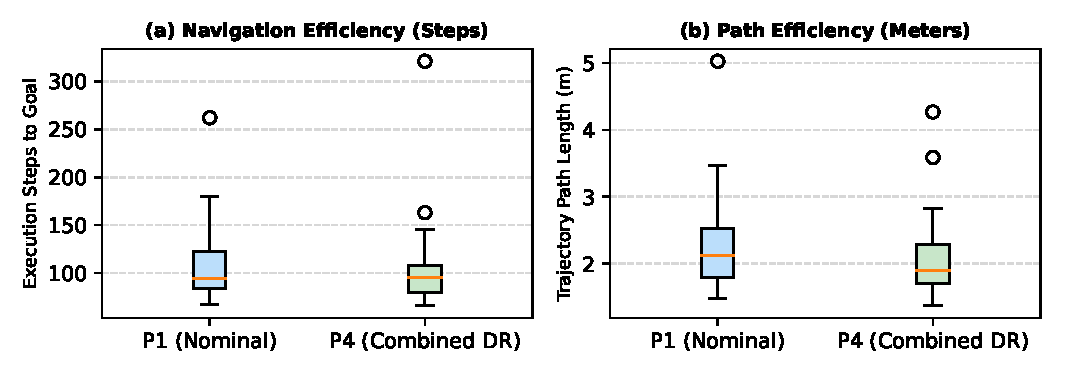
\includegraphics[width=\columnwidth]{figures/fig3_trajectory_metrics.pdf}
\caption{Distribution of navigation efficiency metrics for successful held-out episodes. (a) Execution steps to goal. (b) Trajectory path length in meters.}
\label{fig:boxplots}
\end{figure}

\section{Limitations and Pending Work}

\subsection{Methodological Limitations and Confounders}
Our audit identified three primary methodological confounders:
\begin{enumerate}
    \item \textbf{Unequal Training Budgets:} Due to strict execution deadlines, policy $\text{P1}$ was trained for 852,816 steps, whereas $\text{P4}$ completed 704,512 steps (a 17.4\% reduction). That $\text{P4}$ achieves high nominal success despite fewer steps is consistent with, but does not definitively establish, improved sample efficiency.
    \item \textbf{Single Random Seed:} Completed runs represent a single training seed ($s=0$). Consequently, inter-run training variance cannot currently be quantified.
    \item \textbf{Simulation-Only Scope:} All experiments reflect Gazebo Classic physics. Physical robot validation has not yet been demonstrated.
\end{enumerate}

\begin{table}[t]
\caption{Planned $4 \times 4$ Policy / Environment Cross-Evaluation Matrix}
\centering
\begin{tabular}{lcccc}
\toprule
\textbf{Trained} & \multicolumn{4}{c}{\textbf{Evaluation Environment Condition}} \\
\cmidrule{2-5}
\textbf{Policy} & \textbf{Nominal} & \textbf{Sensor DR} & \textbf{Dynamics DR} & \textbf{Combined DR} \\
\midrule
\textbf{P1 (Nominal)} & Completed (94\%) & Pending & Pending & Pending \\
\textbf{P2 (Sensor)}  & Pending          & Pending & Pending & Pending \\
\textbf{P3 (Dynamics)}& Pending          & Pending & Pending & Pending \\
\textbf{P4 (Combined)}& Completed (98\%) & Pending & Pending & Pending \\
\bottomrule
\end{tabular}
\label{tab:matrix}
\end{table}

\subsection{Pending Work and Project Roadmap}
The remaining project timeline is structured around three core phases:
\begin{enumerate}
    \item \textbf{Ablation Training ($\text{P2}$ and $\text{P3}$):} Train policy $\text{P2}$ (sensor noise only) and policy $\text{P3}$ (dynamics perturbations only) with equalized budgets of 850k steps to isolate parameter impacts.
    \item \textbf{$4 \times 4$ Cross-Evaluation Matrix:} Execute the planned cross-evaluation matrix (Table~\ref{tab:matrix}) assessing each policy against nominal and perturbed conditions to rigorously measure out-of-distribution robustness.
    \item \textbf{Expanded Evaluation ($N=250$):} Scale test scenarios from 50 to 250 diverse test cases across nominal and stress conditions.
    \item \textbf{Physical Robot Deployment:} Deploy policy $\text{P4}$ to a physical TurtleBot3 Burger in a laboratory testing arena, conditional on hardware access, lab availability, and safety approval.
\end{enumerate}

\section{Individual Contributions}
\textit{Both authors contributed to the project with complementary responsibilities. Both authors must confirm the final contribution declaration upon report submission.}

\begin{itemize}
    \item \textbf{Saigirish S (B24ME1066):} Primary reinforcement learning pipeline architecture; implementation of the 43-D observation preprocessor and dead-reckoning module; domain randomization algorithms \cite{tobin2017domain, peng2018sim}; multi-worker Gazebo orchestration; training executions of policies $\text{P1}$ and $\text{P4}$; ROS 2 standalone inference node development.
    \item \textbf{Siddhi Vinayak (B24BB1036):} Reward decomposition audit framework; per-step reward trace logging; unit test execution and baseline validation; participation in experimental design and hardware deployment preparation.
\end{itemize}

\section{Conclusion}
This mid-term progress report presents an initial implementation and evaluation baseline for mapless autonomous navigation using PPO \cite{schulman2017proximal} and domain randomization \cite{tobin2017domain, peng2018sim}. By coupling sector min-pooled LiDAR readings with dead-reckoning goal tracking, the policy achieves high navigation reliability under nominal simulation conditions (94\%--98\% success). Methodological rigor demonstrates that observed preliminary differences between nominal and randomized policies are not statistically significant at $N=50$, establishing a clear requirement for expanded benchmarking and perturbed-environment cross-evaluations. The completed architecture provides a solid trajectory toward completing the planned ablation matrix and physical robot deployment.

\bibliographystyle{IEEEtran}
\bibliography{references}

\end{document}
